\documentclass[handout]{ximera}

\title{Video Set Introduction}

\begin{document}

\begin{abstract}
\end{abstract}

%Vid Set 6

\maketitle


\begin{javascript}
  nameCheck = function(a,b) {
    return a.toLowerCase() != b.toLowerCase();
  };
\end{javascript}

Before watching the video, think about and answer these questions to the best of your ability. Your answer will always be recorded as correct, regardless of your answer choice.

\begin{problem}
Consider the function $f(x) = -x^{2.2}+3x^{1.2}+2$. Use calculus to find the maximum value of $f(x)$ over the interval $[-.75,4]$.
$\answer[format=string,validator=nameCheck]{}$
\end{problem}



\begin{problem}
Consider the graph below. This is the graph of $f'(x)$, the \textbf{derivative} of the function $f(x)$. The labels are naming the $x$-coordinate of each point. The function is not defined for $x$-values less than $x=A$.
\begin{image}
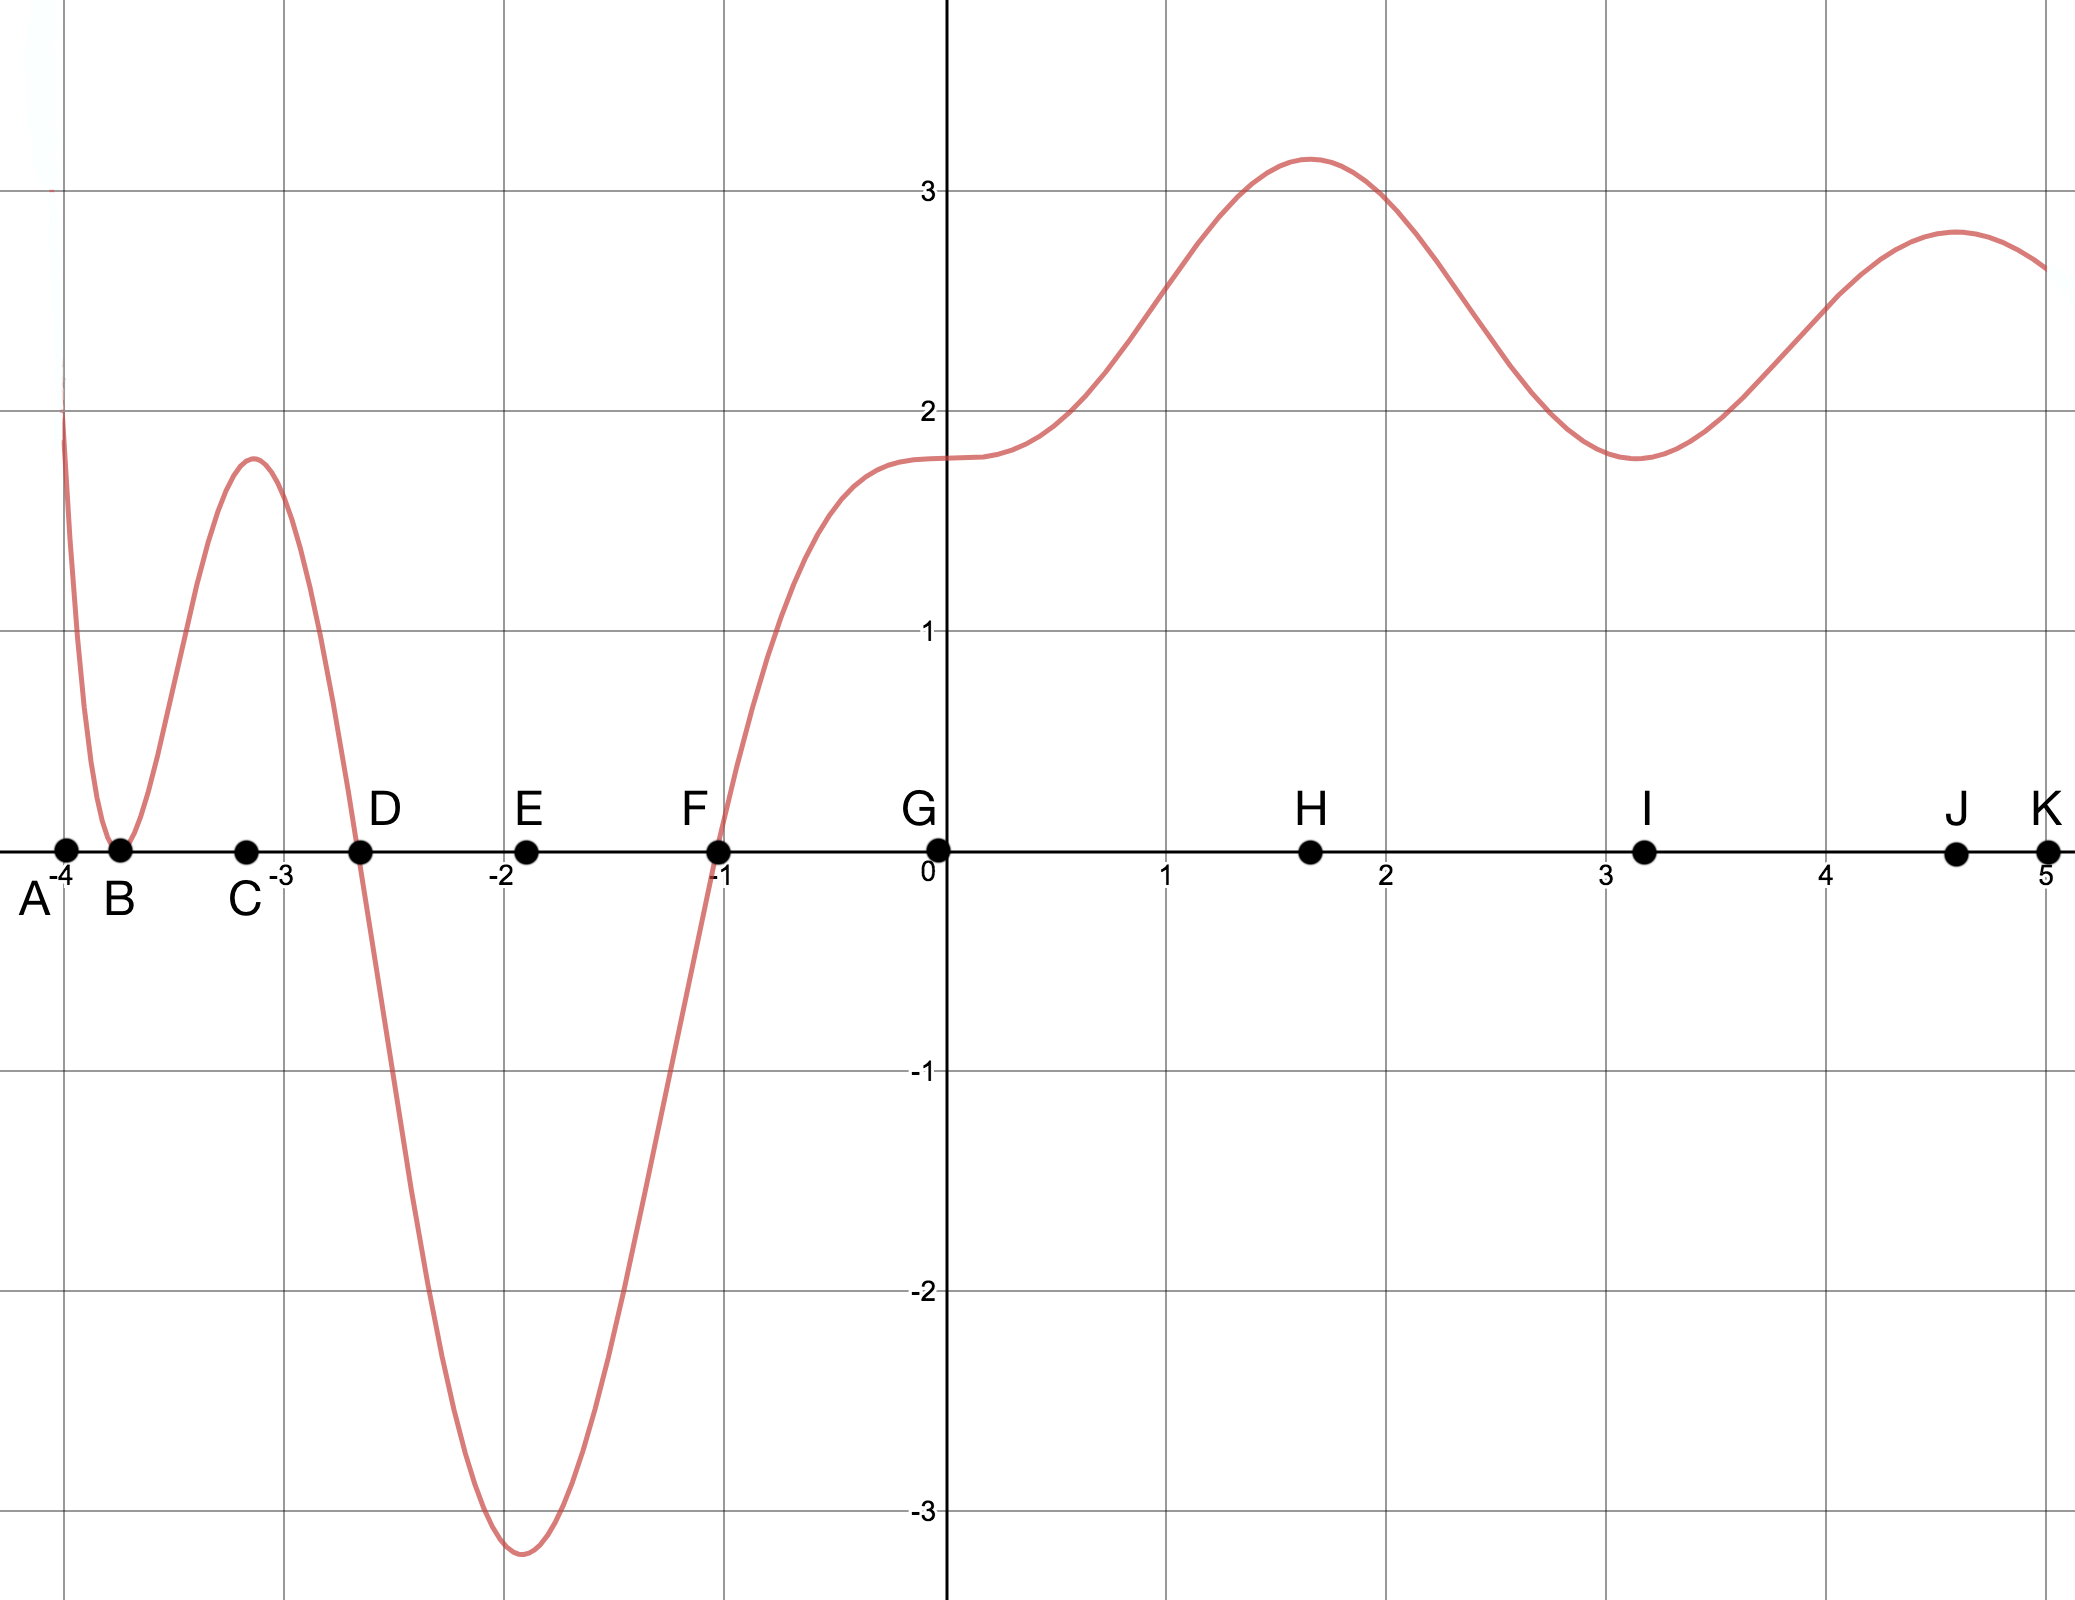
\includegraphics{maxmingraph.png}
\end{image}

In particular, note that:
\begin{itemize}
\item from $x=A$ to $x=B$, $f'(x)>0$ \ \ \ \ \
\item from $x=B$ to $x=C$, $f'(x)>0$
\item from $x=C$ to $x=D$, $f'(x)>0$
\item from $x=D$ to $x=E$, $f'(x)<0$
\item from $x=E$ to $x=F$, $f'(x)<0$
\item from $x=F$ to $x=G$, $f'(x)>0$
\item from $x=G$ to $x=H$, $f'(x)>0$
\item from $x=H$ to $x=I$, $f'(x)>0$
\item from $x=I$ to $x=J$, $f'(x)>0$
\end{itemize}

For each of the points, determine whether they are a maximum, minimum, or neither.

\begin{tabular}{l l l l l}

\begin{minipage}[t]{0.2\textwidth}
At $x=A$, f(x) has a
\begin{multipleChoice}
\choice[correct]{maximum}
\choice[correct]{minimum}
\choice[correct]{neither}
\end{multipleChoice}
\end{minipage} &

\begin{minipage}[t]{0.2\textwidth}
At $x=B$, f(x) has a
\begin{multipleChoice}
\choice[correct]{maximum}
\choice[correct]{minimum}
\choice[correct]{neither}
\end{multipleChoice}
\end{minipage} &

\begin{minipage}[t]{0.2\textwidth}
At $x=C$, f(x) has a
\begin{multipleChoice}
\choice[correct]{maximum}
\choice[correct]{minimum}
\choice[correct]{neither}
\end{multipleChoice}
\end{minipage} &

\begin{minipage}[t]{0.2\textwidth}
At $x=D$, f(x) has a
\begin{multipleChoice}
\choice[correct]{maximum}
\choice[correct]{minimum}
\choice[correct]{neither}
\end{multipleChoice}
\end{minipage} &

\begin{minipage}[t]{0.2\textwidth}
At $x=E$, f(x) has a
\begin{multipleChoice}
\choice[correct]{maximum}
\choice[correct]{minimum}
\choice[correct]{neither}
\end{multipleChoice}
\end{minipage} \\

\begin{minipage}[t]{0.2\textwidth}
At $x=F$, f(x) has a
\begin{multipleChoice}
\choice[correct]{maximum}
\choice[correct]{minimum}
\choice[correct]{neither}
\end{multipleChoice}
\end{minipage} &

\begin{minipage}[t]{0.2\textwidth}
At $x=G$, f(x) has a
\begin{multipleChoice}
\choice[correct]{maximum}
\choice[correct]{minimum}
\choice[correct]{neither}
\end{multipleChoice}
\end{minipage} &

\begin{minipage}[t]{0.2\textwidth}
At $x=H$, f(x) has a
\begin{multipleChoice}
\choice[correct]{maximum}
\choice[correct]{minimum}
\choice[correct]{neither}
\end{multipleChoice}
\end{minipage} &

\begin{minipage}[t]{0.2\textwidth}
At $x=I$, f(x) has a
\begin{multipleChoice}
\choice[correct]{maximum}
\choice[correct]{minimum}
\choice[correct]{neither}
\end{multipleChoice}
\end{minipage} &

\begin{minipage}[t]{0.2\textwidth}
At $x=J$, f(x) has a
\begin{multipleChoice}
\choice[correct]{maximum}
\choice[correct]{minimum}
\choice[correct]{neither}
\end{multipleChoice}
\end{minipage}

\end{tabular}

\end{problem}
\end{document}